% Options for packages loaded elsewhere
\PassOptionsToPackage{unicode}{hyperref}
\PassOptionsToPackage{hyphens}{url}
\PassOptionsToPackage{dvipsnames,svgnames,x11names}{xcolor}
%
\documentclass[
  letterpaper,
  DIV=11,
  numbers=noendperiod]{scrartcl}

\usepackage{amsmath,amssymb}
\usepackage{iftex}
\ifPDFTeX
  \usepackage[T1]{fontenc}
  \usepackage[utf8]{inputenc}
  \usepackage{textcomp} % provide euro and other symbols
\else % if luatex or xetex
  \usepackage{unicode-math}
  \defaultfontfeatures{Scale=MatchLowercase}
  \defaultfontfeatures[\rmfamily]{Ligatures=TeX,Scale=1}
\fi
\usepackage{lmodern}
\ifPDFTeX\else  
    % xetex/luatex font selection
\fi
% Use upquote if available, for straight quotes in verbatim environments
\IfFileExists{upquote.sty}{\usepackage{upquote}}{}
\IfFileExists{microtype.sty}{% use microtype if available
  \usepackage[]{microtype}
  \UseMicrotypeSet[protrusion]{basicmath} % disable protrusion for tt fonts
}{}
\makeatletter
\@ifundefined{KOMAClassName}{% if non-KOMA class
  \IfFileExists{parskip.sty}{%
    \usepackage{parskip}
  }{% else
    \setlength{\parindent}{0pt}
    \setlength{\parskip}{6pt plus 2pt minus 1pt}}
}{% if KOMA class
  \KOMAoptions{parskip=half}}
\makeatother
\usepackage{xcolor}
\setlength{\emergencystretch}{3em} % prevent overfull lines
\setcounter{secnumdepth}{-\maxdimen} % remove section numbering
% Make \paragraph and \subparagraph free-standing
\makeatletter
\ifx\paragraph\undefined\else
  \let\oldparagraph\paragraph
  \renewcommand{\paragraph}{
    \@ifstar
      \xxxParagraphStar
      \xxxParagraphNoStar
  }
  \newcommand{\xxxParagraphStar}[1]{\oldparagraph*{#1}\mbox{}}
  \newcommand{\xxxParagraphNoStar}[1]{\oldparagraph{#1}\mbox{}}
\fi
\ifx\subparagraph\undefined\else
  \let\oldsubparagraph\subparagraph
  \renewcommand{\subparagraph}{
    \@ifstar
      \xxxSubParagraphStar
      \xxxSubParagraphNoStar
  }
  \newcommand{\xxxSubParagraphStar}[1]{\oldsubparagraph*{#1}\mbox{}}
  \newcommand{\xxxSubParagraphNoStar}[1]{\oldsubparagraph{#1}\mbox{}}
\fi
\makeatother

\usepackage{color}
\usepackage{fancyvrb}
\newcommand{\VerbBar}{|}
\newcommand{\VERB}{\Verb[commandchars=\\\{\}]}
\DefineVerbatimEnvironment{Highlighting}{Verbatim}{commandchars=\\\{\}}
% Add ',fontsize=\small' for more characters per line
\usepackage{framed}
\definecolor{shadecolor}{RGB}{241,243,245}
\newenvironment{Shaded}{\begin{snugshade}}{\end{snugshade}}
\newcommand{\AlertTok}[1]{\textcolor[rgb]{0.68,0.00,0.00}{#1}}
\newcommand{\AnnotationTok}[1]{\textcolor[rgb]{0.37,0.37,0.37}{#1}}
\newcommand{\AttributeTok}[1]{\textcolor[rgb]{0.40,0.45,0.13}{#1}}
\newcommand{\BaseNTok}[1]{\textcolor[rgb]{0.68,0.00,0.00}{#1}}
\newcommand{\BuiltInTok}[1]{\textcolor[rgb]{0.00,0.23,0.31}{#1}}
\newcommand{\CharTok}[1]{\textcolor[rgb]{0.13,0.47,0.30}{#1}}
\newcommand{\CommentTok}[1]{\textcolor[rgb]{0.37,0.37,0.37}{#1}}
\newcommand{\CommentVarTok}[1]{\textcolor[rgb]{0.37,0.37,0.37}{\textit{#1}}}
\newcommand{\ConstantTok}[1]{\textcolor[rgb]{0.56,0.35,0.01}{#1}}
\newcommand{\ControlFlowTok}[1]{\textcolor[rgb]{0.00,0.23,0.31}{\textbf{#1}}}
\newcommand{\DataTypeTok}[1]{\textcolor[rgb]{0.68,0.00,0.00}{#1}}
\newcommand{\DecValTok}[1]{\textcolor[rgb]{0.68,0.00,0.00}{#1}}
\newcommand{\DocumentationTok}[1]{\textcolor[rgb]{0.37,0.37,0.37}{\textit{#1}}}
\newcommand{\ErrorTok}[1]{\textcolor[rgb]{0.68,0.00,0.00}{#1}}
\newcommand{\ExtensionTok}[1]{\textcolor[rgb]{0.00,0.23,0.31}{#1}}
\newcommand{\FloatTok}[1]{\textcolor[rgb]{0.68,0.00,0.00}{#1}}
\newcommand{\FunctionTok}[1]{\textcolor[rgb]{0.28,0.35,0.67}{#1}}
\newcommand{\ImportTok}[1]{\textcolor[rgb]{0.00,0.46,0.62}{#1}}
\newcommand{\InformationTok}[1]{\textcolor[rgb]{0.37,0.37,0.37}{#1}}
\newcommand{\KeywordTok}[1]{\textcolor[rgb]{0.00,0.23,0.31}{\textbf{#1}}}
\newcommand{\NormalTok}[1]{\textcolor[rgb]{0.00,0.23,0.31}{#1}}
\newcommand{\OperatorTok}[1]{\textcolor[rgb]{0.37,0.37,0.37}{#1}}
\newcommand{\OtherTok}[1]{\textcolor[rgb]{0.00,0.23,0.31}{#1}}
\newcommand{\PreprocessorTok}[1]{\textcolor[rgb]{0.68,0.00,0.00}{#1}}
\newcommand{\RegionMarkerTok}[1]{\textcolor[rgb]{0.00,0.23,0.31}{#1}}
\newcommand{\SpecialCharTok}[1]{\textcolor[rgb]{0.37,0.37,0.37}{#1}}
\newcommand{\SpecialStringTok}[1]{\textcolor[rgb]{0.13,0.47,0.30}{#1}}
\newcommand{\StringTok}[1]{\textcolor[rgb]{0.13,0.47,0.30}{#1}}
\newcommand{\VariableTok}[1]{\textcolor[rgb]{0.07,0.07,0.07}{#1}}
\newcommand{\VerbatimStringTok}[1]{\textcolor[rgb]{0.13,0.47,0.30}{#1}}
\newcommand{\WarningTok}[1]{\textcolor[rgb]{0.37,0.37,0.37}{\textit{#1}}}

\providecommand{\tightlist}{%
  \setlength{\itemsep}{0pt}\setlength{\parskip}{0pt}}\usepackage{longtable,booktabs,array}
\usepackage{calc} % for calculating minipage widths
% Correct order of tables after \paragraph or \subparagraph
\usepackage{etoolbox}
\makeatletter
\patchcmd\longtable{\par}{\if@noskipsec\mbox{}\fi\par}{}{}
\makeatother
% Allow footnotes in longtable head/foot
\IfFileExists{footnotehyper.sty}{\usepackage{footnotehyper}}{\usepackage{footnote}}
\makesavenoteenv{longtable}
\usepackage{graphicx}
\makeatletter
\def\maxwidth{\ifdim\Gin@nat@width>\linewidth\linewidth\else\Gin@nat@width\fi}
\def\maxheight{\ifdim\Gin@nat@height>\textheight\textheight\else\Gin@nat@height\fi}
\makeatother
% Scale images if necessary, so that they will not overflow the page
% margins by default, and it is still possible to overwrite the defaults
% using explicit options in \includegraphics[width, height, ...]{}
\setkeys{Gin}{width=\maxwidth,height=\maxheight,keepaspectratio}
% Set default figure placement to htbp
\makeatletter
\def\fps@figure{htbp}
\makeatother

\KOMAoption{captions}{tableheading}
\makeatletter
\@ifpackageloaded{caption}{}{\usepackage{caption}}
\AtBeginDocument{%
\ifdefined\contentsname
  \renewcommand*\contentsname{Table of contents}
\else
  \newcommand\contentsname{Table of contents}
\fi
\ifdefined\listfigurename
  \renewcommand*\listfigurename{List of Figures}
\else
  \newcommand\listfigurename{List of Figures}
\fi
\ifdefined\listtablename
  \renewcommand*\listtablename{List of Tables}
\else
  \newcommand\listtablename{List of Tables}
\fi
\ifdefined\figurename
  \renewcommand*\figurename{Figure}
\else
  \newcommand\figurename{Figure}
\fi
\ifdefined\tablename
  \renewcommand*\tablename{Table}
\else
  \newcommand\tablename{Table}
\fi
}
\@ifpackageloaded{float}{}{\usepackage{float}}
\floatstyle{ruled}
\@ifundefined{c@chapter}{\newfloat{codelisting}{h}{lop}}{\newfloat{codelisting}{h}{lop}[chapter]}
\floatname{codelisting}{Listing}
\newcommand*\listoflistings{\listof{codelisting}{List of Listings}}
\makeatother
\makeatletter
\makeatother
\makeatletter
\@ifpackageloaded{caption}{}{\usepackage{caption}}
\@ifpackageloaded{subcaption}{}{\usepackage{subcaption}}
\makeatother

\ifLuaTeX
  \usepackage{selnolig}  % disable illegal ligatures
\fi
\usepackage{bookmark}

\IfFileExists{xurl.sty}{\usepackage{xurl}}{} % add URL line breaks if available
\urlstyle{same} % disable monospaced font for URLs
\hypersetup{
  pdftitle={01 Mini Project: Static Maps},
  pdfauthor={Solveig Senf},
  colorlinks=true,
  linkcolor={blue},
  filecolor={Maroon},
  citecolor={Blue},
  urlcolor={Blue},
  pdfcreator={LaTeX via pandoc}}


\title{01 Mini Project: Static Maps}
\author{Solveig Senf}
\date{}

\begin{document}
\maketitle


This project features three maps (a static and interactive version of
the same variable and a single static map of different variable) that
display data from the Centers for Disease Control and Prevention (CDC).
Data on Covid-19 levels was collected from February 2022 to May 2023 on
a county level. This project displays data recorded on May 11, 2023. For
the purposes of this state-level project, I will use the average of
county-level data for each state to display Covid-19 cases per 100k.
Data can be accessed
\href{https://data.cdc.gov/Public-Health-Surveillance/United-States-COVID-19-Community-Levels-by-County/3nnm-4jni/about_data}{here}.

Additionally, this project contains two maps (a static and interactive
version) that display the 2024 Presidential Election results. Election
data is from the Federal Election Commission (FEC) and can be found at
\href{https://www.fec.gov/introduction-campaign-finance/election-results-and-voting-information/}{this
link}.

\begin{Shaded}
\begin{Highlighting}[]
\FunctionTok{library}\NormalTok{(tidyverse)}
\end{Highlighting}
\end{Shaded}

\begin{verbatim}
-- Attaching core tidyverse packages ------------------------ tidyverse 2.0.0 --
v dplyr     1.1.4     v readr     2.1.5
v forcats   1.0.0     v stringr   1.5.1
v ggplot2   3.5.1     v tibble    3.2.1
v lubridate 1.9.4     v tidyr     1.3.1
v purrr     1.0.4     
-- Conflicts ------------------------------------------ tidyverse_conflicts() --
x dplyr::filter() masks stats::filter()
x dplyr::lag()    masks stats::lag()
i Use the conflicted package (<http://conflicted.r-lib.org/>) to force all conflicts to become errors
\end{verbatim}

\begin{Shaded}
\begin{Highlighting}[]
\FunctionTok{library}\NormalTok{(mdsr)}
\FunctionTok{library}\NormalTok{(maps)}
\end{Highlighting}
\end{Shaded}

\begin{verbatim}

Attaching package: 'maps'

The following object is masked from 'package:purrr':

    map
\end{verbatim}

\begin{Shaded}
\begin{Highlighting}[]
\FunctionTok{library}\NormalTok{(viridis)}
\end{Highlighting}
\end{Shaded}

\begin{verbatim}
Loading required package: viridisLite

Attaching package: 'viridis'

The following object is masked from 'package:maps':

    unemp
\end{verbatim}

\begin{Shaded}
\begin{Highlighting}[]
\FunctionTok{library}\NormalTok{(lubridate)}
\FunctionTok{library}\NormalTok{(leaflet)}
\FunctionTok{library}\NormalTok{(sf)}
\end{Highlighting}
\end{Shaded}

\begin{verbatim}
Linking to GEOS 3.11.0, GDAL 3.5.3, PROJ 9.1.0; sf_use_s2() is TRUE
\end{verbatim}

\begin{Shaded}
\begin{Highlighting}[]
\FunctionTok{library}\NormalTok{(RColorBrewer)}
\end{Highlighting}
\end{Shaded}

COVID-19 Data

\begin{Shaded}
\begin{Highlighting}[]
\CommentTok{\#data set from the CDC}
\NormalTok{cdc\_data }\OtherTok{\textless{}{-}} \FunctionTok{read.csv}\NormalTok{(}\StringTok{"\textasciitilde{}/Downloads/01\_United\_States\_COVID{-}19\_Community\_Levels\_by\_County\_20250216.csv"}\NormalTok{)}
\end{Highlighting}
\end{Shaded}

\begin{Shaded}
\begin{Highlighting}[]
\NormalTok{covid\_data }\OtherTok{\textless{}{-}}\NormalTok{ cdc\_data }\SpecialCharTok{|\textgreater{}}
  \FunctionTok{filter}\NormalTok{(date\_updated }\SpecialCharTok{==} \StringTok{"2023{-}05{-}11"}\NormalTok{, }
         \SpecialCharTok{!}\NormalTok{(state }\SpecialCharTok{\%in\%} \FunctionTok{c}\NormalTok{(}\StringTok{"Puerto Rico"}\NormalTok{, }
                        \StringTok{"American Samoa"}\NormalTok{, }
                        \StringTok{"Commonwealth of the Northern Mariana Islands"}\NormalTok{, }
                        \StringTok{"United States Virgin Islands"}\NormalTok{, }
                        \StringTok{"Guam"}\NormalTok{)))}
\end{Highlighting}
\end{Shaded}

\begin{Shaded}
\begin{Highlighting}[]
\NormalTok{states\_polygon }\OtherTok{\textless{}{-}} \FunctionTok{as\_tibble}\NormalTok{(}\FunctionTok{map\_data}\NormalTok{(}\StringTok{"state"}\NormalTok{)) }\SpecialCharTok{|\textgreater{}}
  \FunctionTok{select}\NormalTok{(region, group, order, lat, long)}

\NormalTok{states\_sf }\OtherTok{\textless{}{-}} \FunctionTok{read\_sf}\NormalTok{(}\StringTok{"https://rstudio.github.io/leaflet/json/us{-}states.geojson"}\NormalTok{) }\SpecialCharTok{|\textgreater{}}
  \FunctionTok{select}\NormalTok{(name, geometry)}
\end{Highlighting}
\end{Shaded}

\begin{Shaded}
\begin{Highlighting}[]
\CommentTok{\#convert county{-}level data to state{-}level data}
\NormalTok{covid\_state\_level\_data }\OtherTok{\textless{}{-}}\NormalTok{ covid\_data }\SpecialCharTok{|\textgreater{}}
  \FunctionTok{filter}\NormalTok{(covid\_cases\_per\_100k }\SpecialCharTok{!=} \StringTok{"NA"}\NormalTok{) }\SpecialCharTok{|\textgreater{}}
  \FunctionTok{group\_by}\NormalTok{(state) }\SpecialCharTok{|\textgreater{}}
  \FunctionTok{summarize}\NormalTok{(}\AttributeTok{covid\_cases\_per\_100k =} \FunctionTok{mean}\NormalTok{(covid\_cases\_per\_100k))}
\end{Highlighting}
\end{Shaded}

\begin{Shaded}
\begin{Highlighting}[]
\CommentTok{\#format state names in all data sets so they match }
\NormalTok{covid\_state\_level\_data }\OtherTok{\textless{}{-}}\NormalTok{ covid\_state\_level\_data }\SpecialCharTok{|\textgreater{}}
  \FunctionTok{mutate}\NormalTok{(}\AttributeTok{state =} \FunctionTok{str\_to\_lower}\NormalTok{(state),}
         \AttributeTok{state =} \FunctionTok{str\_replace\_all}\NormalTok{(state, }\StringTok{" "}\NormalTok{, }\StringTok{""}\NormalTok{),}
         \AttributeTok{state =} \FunctionTok{str\_squish}\NormalTok{(state))}

\NormalTok{states\_sf }\OtherTok{\textless{}{-}}\NormalTok{ states\_sf }\SpecialCharTok{|\textgreater{}}
  \FunctionTok{mutate}\NormalTok{(}\AttributeTok{name =} \FunctionTok{str\_to\_lower}\NormalTok{(name),}
         \AttributeTok{name =} \FunctionTok{str\_replace\_all}\NormalTok{(name, }\StringTok{" "}\NormalTok{, }\StringTok{""}\NormalTok{))}

\NormalTok{states\_polygon }\OtherTok{\textless{}{-}}\NormalTok{ states\_polygon}\SpecialCharTok{|\textgreater{}}
  \FunctionTok{mutate}\NormalTok{(}\AttributeTok{region =} \FunctionTok{str\_replace\_all}\NormalTok{(region, }\StringTok{" "}\NormalTok{, }\StringTok{""}\NormalTok{))}
\end{Highlighting}
\end{Shaded}

\begin{Shaded}
\begin{Highlighting}[]
\CommentTok{\#join covid data with map data}
\NormalTok{covid\_map }\OtherTok{\textless{}{-}}\NormalTok{ covid\_state\_level\_data }\SpecialCharTok{|\textgreater{}}
  \FunctionTok{right\_join}\NormalTok{(states\_polygon, }\AttributeTok{by =}\FunctionTok{c}\NormalTok{(}\StringTok{"state"} \OtherTok{=} \StringTok{"region"}\NormalTok{))}

\NormalTok{covid\_map }\OtherTok{\textless{}{-}}\NormalTok{ covid\_map }\SpecialCharTok{|\textgreater{}}
  \FunctionTok{right\_join}\NormalTok{(states\_sf, }\AttributeTok{by =}\FunctionTok{c}\NormalTok{(}\StringTok{"state"} \OtherTok{=} \StringTok{"name"}\NormalTok{))}
\end{Highlighting}
\end{Shaded}

Static Map \#1

\begin{Shaded}
\begin{Highlighting}[]
\NormalTok{covid\_map }\SpecialCharTok{|\textgreater{}}
  \FunctionTok{ggplot}\NormalTok{(}\AttributeTok{mapping =} \FunctionTok{aes}\NormalTok{(}\AttributeTok{x =}\NormalTok{ long, }\AttributeTok{y =}\NormalTok{ lat,}
                       \AttributeTok{group =}\NormalTok{ group)) }\SpecialCharTok{+}
  \FunctionTok{geom\_polygon}\NormalTok{(}\FunctionTok{aes}\NormalTok{(}\AttributeTok{fill =}\NormalTok{ covid\_cases\_per\_100k), }\AttributeTok{color =} \StringTok{"white"}\NormalTok{, }\AttributeTok{linewidth =} \FloatTok{0.2}\NormalTok{) }\SpecialCharTok{+}
  \FunctionTok{labs}\NormalTok{(}\AttributeTok{fill =} \StringTok{"Number of Cases"}\NormalTok{,}
       \AttributeTok{x =} \StringTok{""}\NormalTok{,}
       \AttributeTok{y =} \StringTok{""}\NormalTok{,}
       \AttributeTok{title =} \StringTok{"Average number of COVID{-}19 Cases Per 100,000 People"}\NormalTok{,}
       \AttributeTok{subtitle =} \StringTok{"As of May 11, 2023"}\NormalTok{) }\SpecialCharTok{+}
  \FunctionTok{coord\_map}\NormalTok{() }\SpecialCharTok{+}
  \FunctionTok{theme\_void}\NormalTok{() }\SpecialCharTok{+}
  \FunctionTok{scale\_fill\_viridis}\NormalTok{(}\AttributeTok{option =} \StringTok{"mako"}\NormalTok{, }\AttributeTok{direction =} \SpecialCharTok{{-}}\DecValTok{1}\NormalTok{)}
\end{Highlighting}
\end{Shaded}

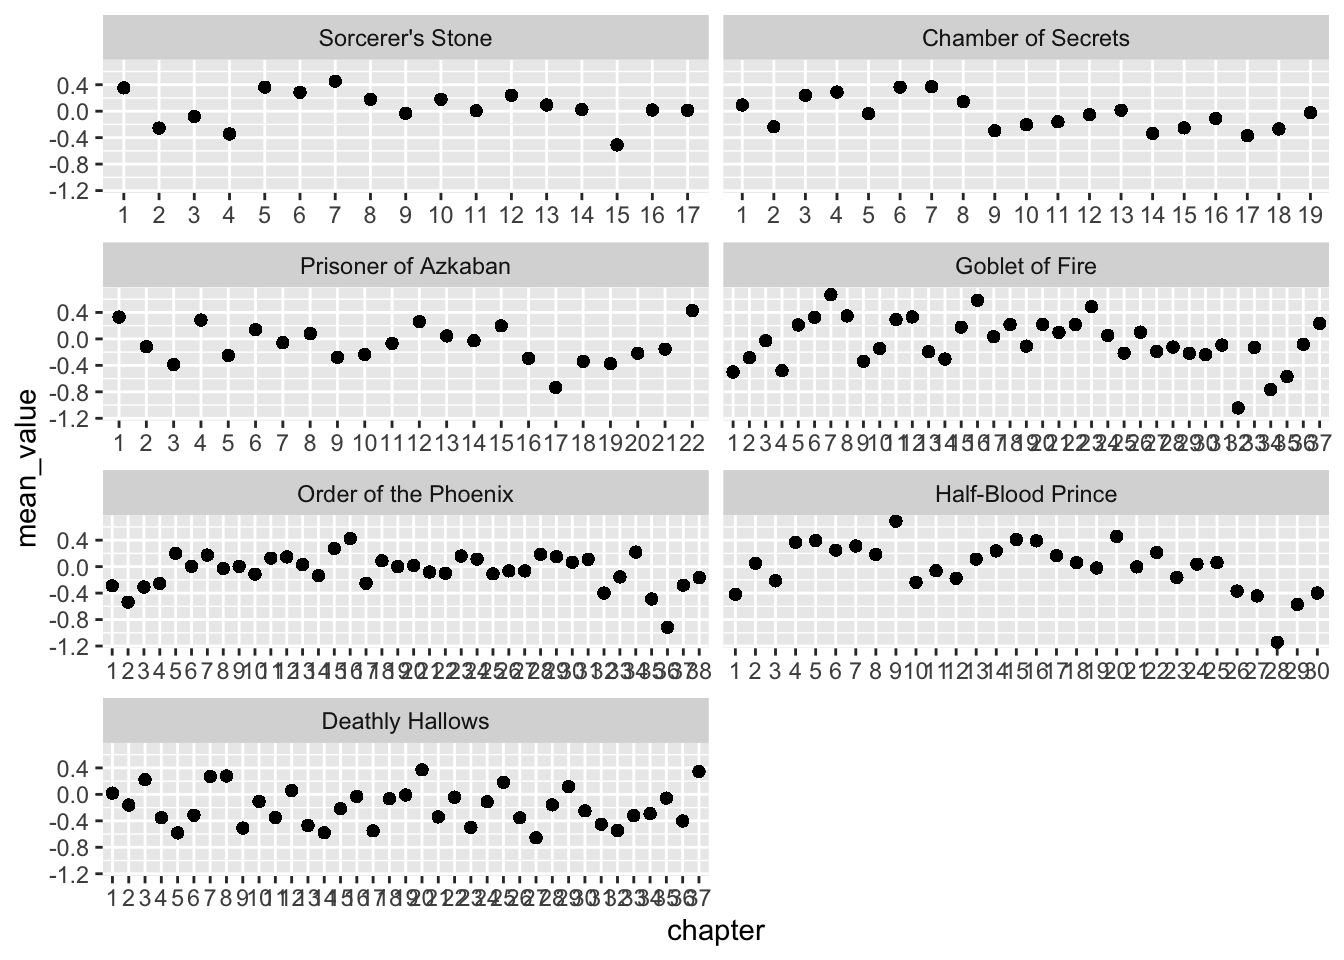
\includegraphics{01_mini_project_static_maps_files/figure-pdf/unnamed-chunk-8-1.pdf}

Static Map \#2

\begin{Shaded}
\begin{Highlighting}[]
\NormalTok{county\_map }\OtherTok{\textless{}{-}} \FunctionTok{map\_data}\NormalTok{(}\StringTok{"county"}\NormalTok{) }\SpecialCharTok{|\textgreater{}}
  \FunctionTok{mutate}\NormalTok{(}\AttributeTok{subregion =} \FunctionTok{str\_to\_lower}\NormalTok{(subregion),}
         \AttributeTok{subregion =} \FunctionTok{str\_replace\_all}\NormalTok{(subregion, }\StringTok{" "}\NormalTok{, }\StringTok{""}\NormalTok{),}
         \AttributeTok{subregion =} \FunctionTok{str\_squish}\NormalTok{(subregion)) }\SpecialCharTok{|\textgreater{}}
  \FunctionTok{mutate}\NormalTok{(}\AttributeTok{region =} \FunctionTok{str\_to\_lower}\NormalTok{(region),}
         \AttributeTok{region =} \FunctionTok{str\_replace\_all}\NormalTok{(region, }\StringTok{" "}\NormalTok{, }\StringTok{""}\NormalTok{))}

\CommentTok{\#fixing odd formating for county names in CDC data}
\NormalTok{covid\_data\_clean }\OtherTok{\textless{}{-}}\NormalTok{ covid\_data }\SpecialCharTok{|\textgreater{}}
  \FunctionTok{select}\NormalTok{(county, state, covid}\FloatTok{.19}\NormalTok{\_community\_level, covid\_cases\_per\_100k) }\SpecialCharTok{|\textgreater{}}
  \FunctionTok{mutate}\NormalTok{(}\AttributeTok{state =} \FunctionTok{str\_to\_lower}\NormalTok{(state),}
         \AttributeTok{state =} \FunctionTok{str\_replace\_all}\NormalTok{(state, }\StringTok{" "}\NormalTok{, }\StringTok{""}\NormalTok{),}
         \AttributeTok{state =} \FunctionTok{str\_squish}\NormalTok{(state)) }\SpecialCharTok{|\textgreater{}}
  \FunctionTok{mutate}\NormalTok{(}\AttributeTok{county =} \FunctionTok{str\_to\_lower}\NormalTok{(county),}
         \AttributeTok{county =} \FunctionTok{str\_replace\_all}\NormalTok{(county, }\StringTok{" "}\NormalTok{, }\StringTok{""}\NormalTok{),}
         \AttributeTok{county =} \FunctionTok{str\_squish}\NormalTok{(county),}
         \AttributeTok{county =} \FunctionTok{str\_replace\_all}\NormalTok{(county, }\StringTok{"county"}\NormalTok{, }\StringTok{""}\NormalTok{),}
         \AttributeTok{county =} \FunctionTok{str\_replace\_all}\NormalTok{(county, }\StringTok{"st."}\NormalTok{, }\StringTok{""}\NormalTok{),}
         \AttributeTok{county =} \FunctionTok{str\_replace\_all}\NormalTok{(county, }\StringTok{"city"}\NormalTok{, }\StringTok{""}\NormalTok{),}
         \AttributeTok{county =} \FunctionTok{str\_replace\_all}\NormalTok{(county, }\StringTok{"muni"}\NormalTok{, }\StringTok{""}\NormalTok{),}
         \AttributeTok{county =} \FunctionTok{str\_replace\_all}\NormalTok{(county, }\StringTok{"parish"}\NormalTok{, }\StringTok{""}\NormalTok{))}

\NormalTok{covid\_county\_level\_data }\OtherTok{\textless{}{-}}\NormalTok{ covid\_data\_clean }\SpecialCharTok{|\textgreater{}}
  \FunctionTok{right\_join}\NormalTok{(county\_map, }\AttributeTok{by =}\FunctionTok{c}\NormalTok{(}\StringTok{"county"} \OtherTok{=} \StringTok{"subregion"}\NormalTok{, }\StringTok{"state"} \OtherTok{=} \StringTok{"region"}\NormalTok{)) }\SpecialCharTok{|\textgreater{}}
  \FunctionTok{mutate}\NormalTok{(}\AttributeTok{covid.19\_community\_level =} \FunctionTok{fct\_relevel}\NormalTok{(covid}\FloatTok{.19}\NormalTok{\_community\_level, }\StringTok{"High"}\NormalTok{, }\StringTok{"Medium"}\NormalTok{, }\StringTok{"Low"}\NormalTok{))}
\end{Highlighting}
\end{Shaded}

\begin{verbatim}
Warning in right_join(covid_data_clean, county_map, by = c(county = "subregion", : Detected an unexpected many-to-many relationship between `x` and `y`.
i Row 1 of `x` matches multiple rows in `y`.
i Row 79510 of `y` matches multiple rows in `x`.
i If a many-to-many relationship is expected, set `relationship =
  "many-to-many"` to silence this warning.
\end{verbatim}

\begin{Shaded}
\begin{Highlighting}[]
\NormalTok{covid\_county\_level\_data }\SpecialCharTok{|\textgreater{}}
  \FunctionTok{ggplot}\NormalTok{(}\AttributeTok{mapping =} \FunctionTok{aes}\NormalTok{(}\AttributeTok{x =}\NormalTok{ long, }\AttributeTok{y =}\NormalTok{ lat,}
                       \AttributeTok{group =}\NormalTok{ group)) }\SpecialCharTok{+}
  \FunctionTok{geom\_polygon}\NormalTok{(}\FunctionTok{aes}\NormalTok{(}\AttributeTok{fill =}\NormalTok{ covid}\FloatTok{.19}\NormalTok{\_community\_level), }\AttributeTok{color =} \StringTok{"white"}\NormalTok{, }\AttributeTok{linewidth =} \FloatTok{0.05}\NormalTok{) }\SpecialCharTok{+}
  \FunctionTok{labs}\NormalTok{(}\AttributeTok{fill =} \StringTok{"Covid Level"}\NormalTok{,}
       \AttributeTok{x =} \StringTok{""}\NormalTok{,}
       \AttributeTok{y =} \StringTok{""}\NormalTok{,}
       \AttributeTok{title =} \StringTok{"COVID{-}19 Levels In Each County"}\NormalTok{,}
       \AttributeTok{subtitle =} \StringTok{"As of May 11, 2023"}\NormalTok{) }\SpecialCharTok{+}
  \FunctionTok{scale\_fill\_manual}\NormalTok{(}\AttributeTok{values =} \FunctionTok{c}\NormalTok{(}\StringTok{"High"} \OtherTok{=} \StringTok{"darkred"}\NormalTok{, }\StringTok{"Medium"} \OtherTok{=} \StringTok{"gold"}\NormalTok{, }\StringTok{"Low"} \OtherTok{=} \StringTok{"darkgreen"}\NormalTok{, }\StringTok{"NA"} \OtherTok{=} \StringTok{"gray"}\NormalTok{)) }\SpecialCharTok{+}
  \FunctionTok{coord\_map}\NormalTok{() }\SpecialCharTok{+}
  \FunctionTok{theme\_void}\NormalTok{() }
\end{Highlighting}
\end{Shaded}

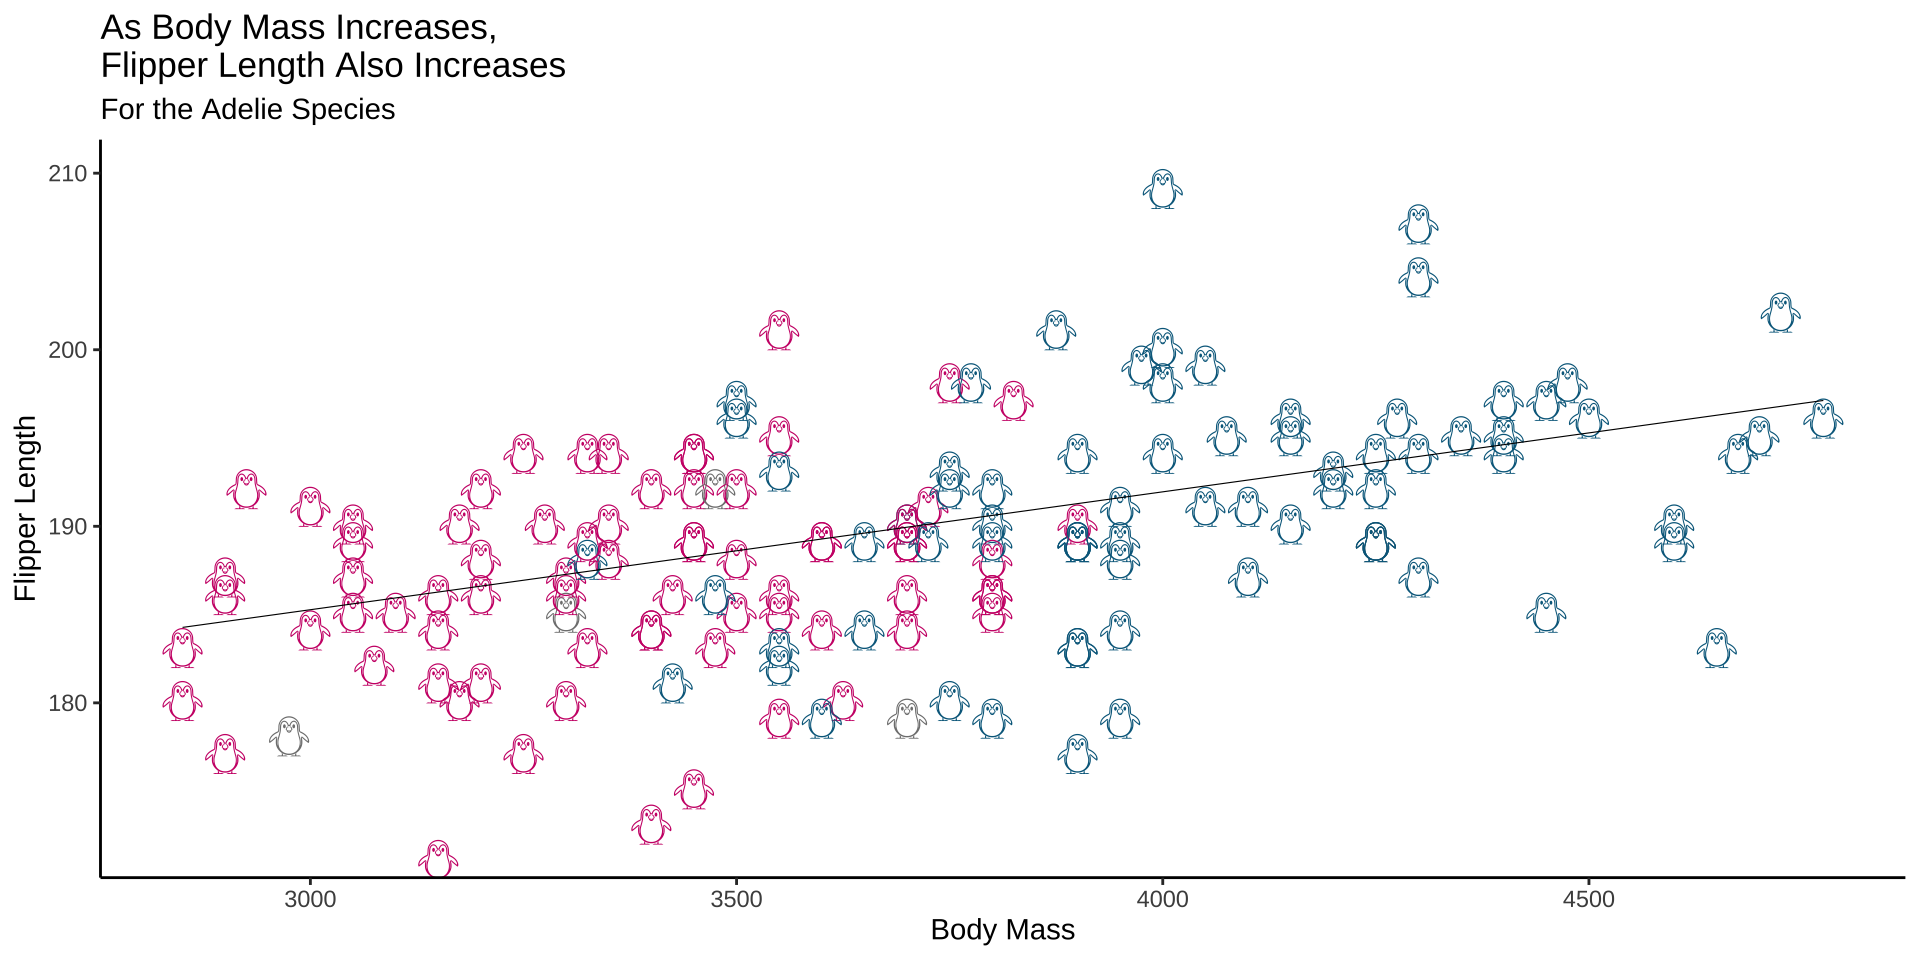
\includegraphics{01_mini_project_static_maps_files/figure-pdf/unnamed-chunk-9-1.pdf}

Election Data

Static Map \#3

\begin{Shaded}
\begin{Highlighting}[]
\CommentTok{\#data from the federal election commission}
\NormalTok{election\_data }\OtherTok{\textless{}{-}} \FunctionTok{read.csv}\NormalTok{(}\StringTok{"\textasciitilde{}/Downloads/2024presgeresults.csv"}\NormalTok{)}

\NormalTok{election\_data }\OtherTok{\textless{}{-}}\NormalTok{ election\_data }\SpecialCharTok{|\textgreater{}}
  \FunctionTok{select}\NormalTok{(STATE, ELECTORAL.VOTE..TRUMP..R., ELECTORAL.VOTE..HARRIS..D., HARRIS, TRUMP) }\SpecialCharTok{|\textgreater{}}
  \FunctionTok{rename}\NormalTok{(}\AttributeTok{state =}\NormalTok{ STATE, }
         \AttributeTok{Trump =}\NormalTok{ ELECTORAL.VOTE..TRUMP..R., }
         \AttributeTok{Harris =}\NormalTok{ ELECTORAL.VOTE..HARRIS..D.,}
         \AttributeTok{votes\_harris =}\NormalTok{ HARRIS,}
         \AttributeTok{votes\_trump =}\NormalTok{ TRUMP) }\SpecialCharTok{|\textgreater{}}
  \FunctionTok{pivot\_longer}\NormalTok{(}\AttributeTok{cols =} \FunctionTok{c}\NormalTok{(Trump, Harris),}
               \AttributeTok{names\_to =}\StringTok{"candidate\_won"}\NormalTok{,}
               \AttributeTok{values\_to =} \StringTok{"electoral\_votes"}\NormalTok{) }\SpecialCharTok{|\textgreater{}}
  \FunctionTok{filter}\NormalTok{(electoral\_votes }\SpecialCharTok{!=} \StringTok{"NA"}\NormalTok{) }\SpecialCharTok{|\textgreater{}} \CommentTok{\#remove observations that show the loosing candidate in each state}
  \FunctionTok{slice}\NormalTok{(}\SpecialCharTok{{-}}\DecValTok{30}\NormalTok{, }\SpecialCharTok{{-}}\DecValTok{20}\NormalTok{) }
\CommentTok{\#slice to remove rows 30 and 20 which are second observations of maine and nebraska due to the fact that they split electoral votes}
\CommentTok{\#the observation recording the winning candidate is kept. }

\NormalTok{election\_data }\OtherTok{\textless{}{-}}\NormalTok{ election\_data }\SpecialCharTok{|\textgreater{}}
  \FunctionTok{mutate}\NormalTok{(}\AttributeTok{state =} \FunctionTok{str\_to\_lower}\NormalTok{(state),}
         \AttributeTok{state =} \FunctionTok{str\_replace\_all}\NormalTok{(state, }\StringTok{" "}\NormalTok{, }\StringTok{""}\NormalTok{),}
         \AttributeTok{state =} \FunctionTok{str\_squish}\NormalTok{(state)) }\SpecialCharTok{|\textgreater{}}
  \FunctionTok{mutate}\NormalTok{(}\AttributeTok{votes\_harris =} \FunctionTok{str\_squish}\NormalTok{(votes\_harris),}
         \AttributeTok{votes\_trump =} \FunctionTok{str\_squish}\NormalTok{(votes\_trump))}
\end{Highlighting}
\end{Shaded}

\begin{Shaded}
\begin{Highlighting}[]
\NormalTok{electoral\_map }\OtherTok{\textless{}{-}}\NormalTok{ election\_data }\SpecialCharTok{|\textgreater{}}
  \FunctionTok{right\_join}\NormalTok{(states\_polygon, }\AttributeTok{by =}\FunctionTok{c}\NormalTok{(}\StringTok{"state"} \OtherTok{=} \StringTok{"region"}\NormalTok{))}

\NormalTok{electoral\_map }\OtherTok{\textless{}{-}}\NormalTok{ electoral\_map }\SpecialCharTok{|\textgreater{}}
  \FunctionTok{right\_join}\NormalTok{(states\_sf, }\AttributeTok{by =}\FunctionTok{c}\NormalTok{(}\StringTok{"state"} \OtherTok{=} \StringTok{"name"}\NormalTok{))}
\end{Highlighting}
\end{Shaded}

\begin{Shaded}
\begin{Highlighting}[]
\NormalTok{electoral\_map }\SpecialCharTok{|\textgreater{}}
  \FunctionTok{ggplot}\NormalTok{(}\AttributeTok{mapping =} \FunctionTok{aes}\NormalTok{(}\AttributeTok{x =}\NormalTok{ long, }\AttributeTok{y =}\NormalTok{ lat,}
                       \AttributeTok{group =}\NormalTok{ group)) }\SpecialCharTok{+}
  \FunctionTok{geom\_polygon}\NormalTok{(}\FunctionTok{aes}\NormalTok{(}\AttributeTok{fill =}\NormalTok{ candidate\_won), }\AttributeTok{color =} \StringTok{"white"}\NormalTok{, }\AttributeTok{linewidth =} \FloatTok{0.2}\NormalTok{) }\SpecialCharTok{+}
  \FunctionTok{labs}\NormalTok{(}\AttributeTok{fill =} \StringTok{"Winning Candidate"}\NormalTok{,}
       \AttributeTok{x =} \StringTok{""}\NormalTok{,}
       \AttributeTok{y =} \StringTok{""}\NormalTok{,}
       \AttributeTok{title =} \StringTok{"2024 Presidential Election Electoral College Map"}\NormalTok{) }\SpecialCharTok{+}
  \FunctionTok{coord\_map}\NormalTok{() }\SpecialCharTok{+}
  \FunctionTok{scale\_fill\_manual}\NormalTok{(}\AttributeTok{values =} \FunctionTok{c}\NormalTok{(}\StringTok{"Harris"} \OtherTok{=} \StringTok{"darkblue"}\NormalTok{, }\StringTok{"Trump"} \OtherTok{=} \StringTok{"darkred"}\NormalTok{)) }\SpecialCharTok{+}
  \FunctionTok{theme\_void}\NormalTok{()}
\end{Highlighting}
\end{Shaded}

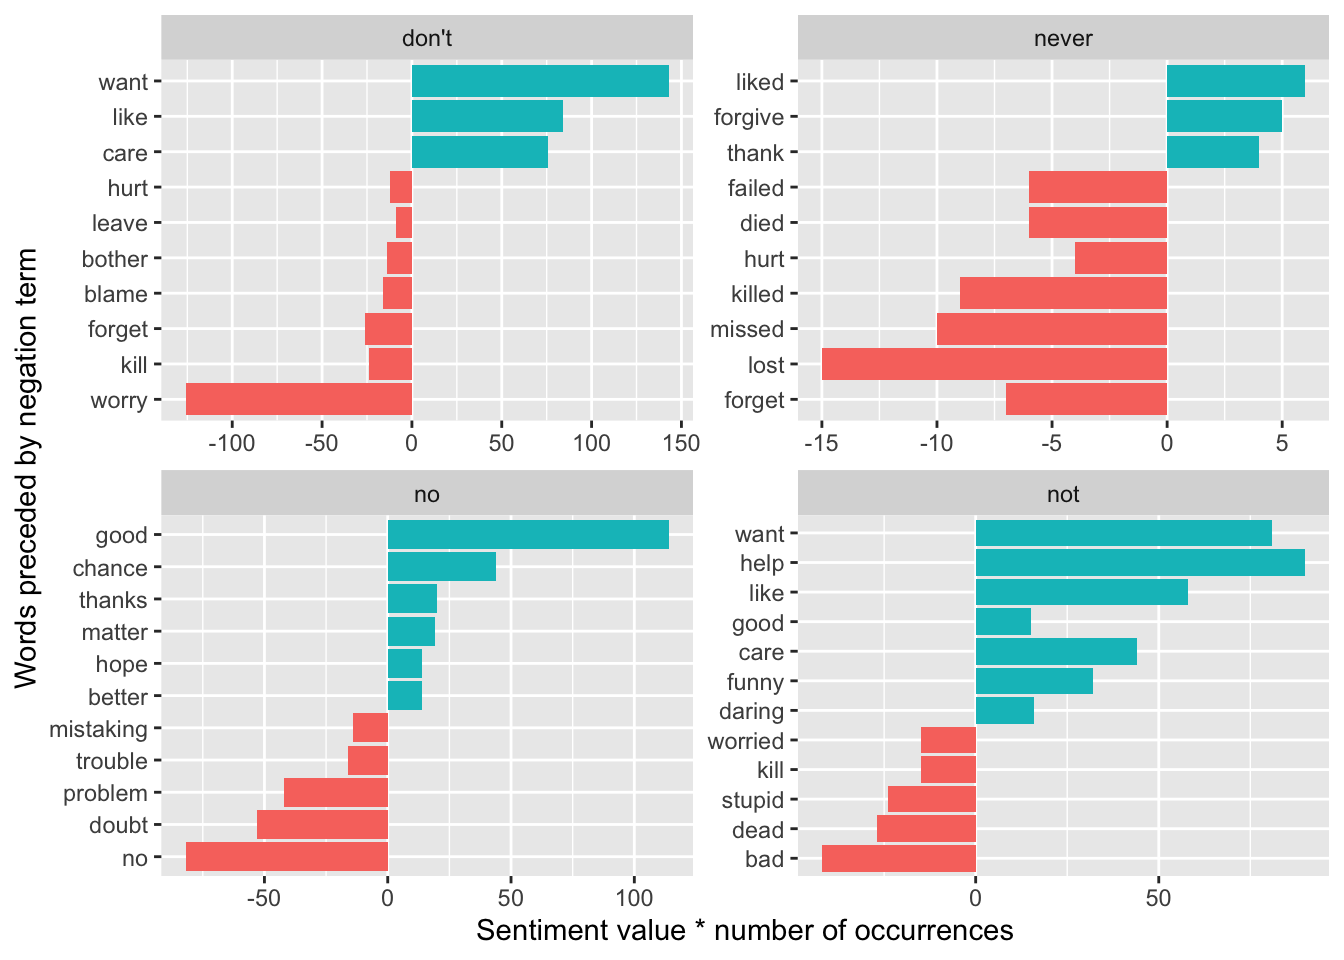
\includegraphics{01_mini_project_static_maps_files/figure-pdf/unnamed-chunk-12-1.pdf}




\end{document}
